\subsection{Radiation}
\label{sec:Radiation Results Discussion}

\subsubsection{Cosmic Radiation}
	The MiniPIX proved to be a reliable way to monitor cosmic radiation levels affecting our payload. Ultimately, we were able to provide a complete profile of atmospheric radiation via the count of hits on the detector and the total absorbed dose. Through morphological analysis we were able to categorize the hits on the detectors and make observations about the variations in secondary vs. primary cosmic rays as our payload passed through the peak layer of ionizing radiation in the stratosphere.

	As displayed in Figure~\ref{fig:hits3}, the MiniPix was able to provide measurements of dosage from cosmic radiation during ascent and during the duration of the time at float. Determining dose rates from the detector was fairly straightforward and from our analysis fairly accurate. Although it would be difficult to directly quantify how accurate this dosage information is we can at the very least conclude that we received similar data to other flights at similar lattitudes.	

\subsubsection{Heat Sink Performance}
%discuss what went well
As Figure \ref{fig:mp_pi_temps} shows, the MiniPIX temperature remained within the operating temperature of the device (\SIrange{0}{70}{\celsius}) throughout the entire flight. This proves the effectiveness of the aluminum heat sink used on the MiniPIX and the \SI{2}{\second} cooldown periods in-between acquisitions. Shortly after the payload was powered on, the internal and external temperatures went through a permanent inversion where the external temperature remained higher than the internal temperature for the remainder of the flight (this cannot be seen in Figure~\ref{fig:mp_pi_temps} due to the \num{225} period moving average). This behavior was seen during the integration/testing phase of construction in Palestine, TX, where the internal temperature remained higher than the external temperature during the entirety of the thermal vacuum testing. Temperature data from integration is shown in Figure~\ref{fig:minipix_integration}. The cause of this is suspected to be due to the placement of our external temperature sensor. The temperature sensor used to measure the external temperature of the MiniPIX is on the same end as the USB connection, where the power dissipation is \SI{2.5}{\watt}, according to the MiniPIX datasheet~\cite{mpdatasheet}. The internal temperature was measured on the same side as the silicon chip, where the power dissipation has a \textit{maximum} value of \SI{2.0}{\watt}, according to the equation $P = IV$ where $P$ is power, $I$ is current, and $V$ is voltage. The silicon chip and the USB connection are on opposite ends of the device, resulting in a temperature gradient. Lastly, the MiniPIX remained powered on and operated during the entire flight, providing consistent acquisition of data across across the entire flight. 

\begin{figure}
  \begin{center}
    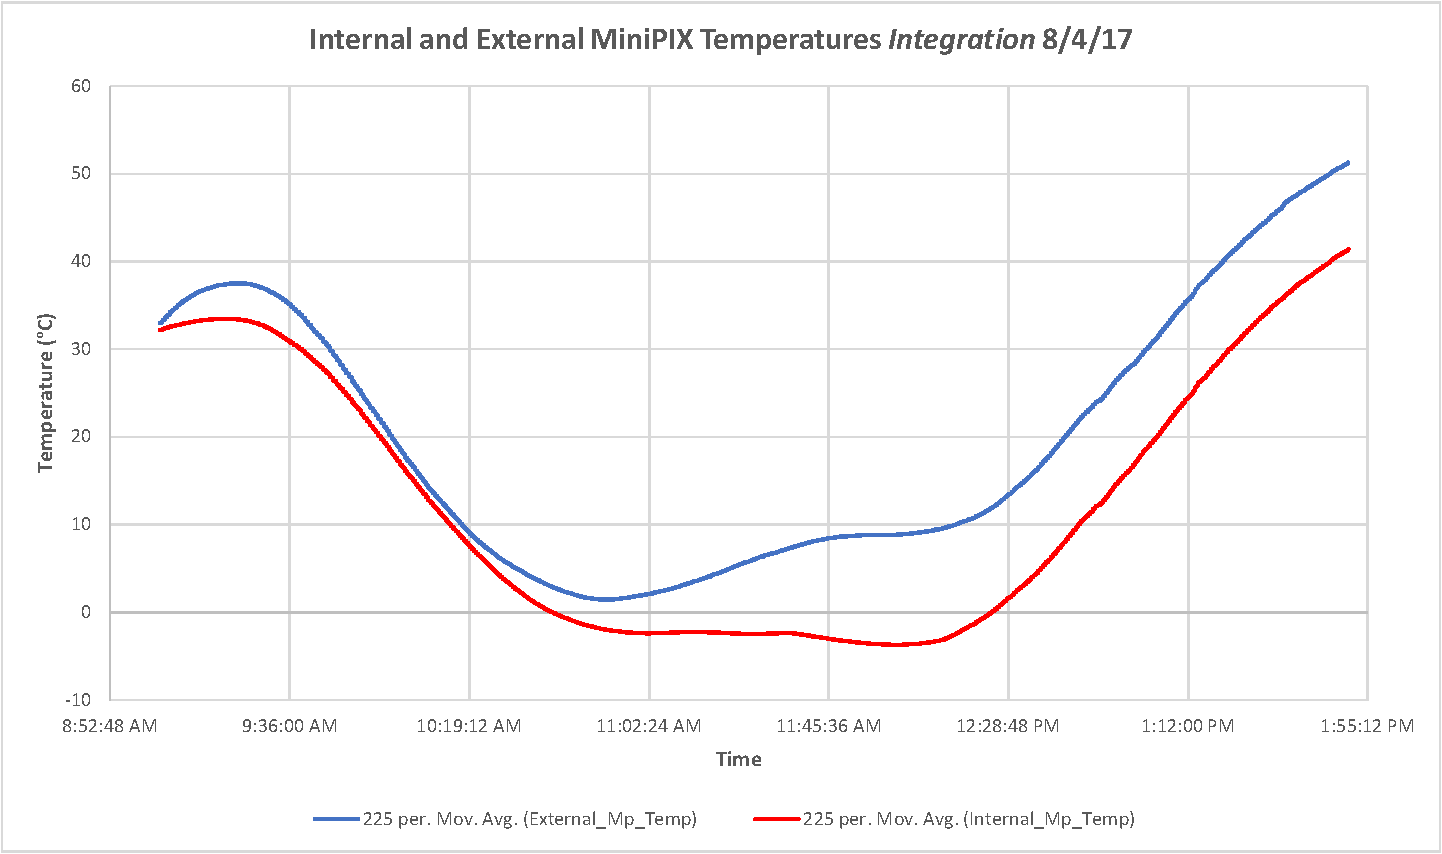
\includegraphics[width=.8\textwidth]{./Figures/integration_temps.pdf}
    \caption{Internal and external MiniPIX temperatures during integration, showing the temperature inversion.}
    \label{fig:minipix_integration}
  \end{center}
\end{figure}



%discuss what we learned and how we will do it better
%expand on issues listed before


%discuss the additional findings such as the Maximum-event Andrew researched

%inside \ref{fig:LABEL NAME}



\subsubsection{Solar UV Radiation}

The photodiodes used in this experiment recorded reasonably accurate data of the solar UV spectrum during the high-altitude flight, as they produce little to no dark current. However, due to limitations of the detector, we have concluded that this device is not suitable for making precise measurements of UV irradiance. As the device is used over time, the responsivity of the detector decreases. Additionally, each time the photodiodes are saturated, the responsivity of the sensor decreases. These effects are unavoidable since the photodiodes must be tested to ensure they are functioning properly and deliver the correct data. During our testing, one photodiode may have been saturated more times than the others, or perhaps one experienced more exposure time overall during testing than the others. This effect has been attributed to the unusual behavior seen in the data collected by sensors UV$_1$ and UV$_2$. The peak irradiance recorded by UV$_1$ is considerably lower than UV$_0$. Similarly, the peak for UV$_2$ is lower than the other two. Another thing to note is that the UV$_2$ data doesn't begin at \SI{0.00}{\watt\per\meter\squared} like the data from UV$_0$ and UV$_1$. This is either due to the decrease in responsivity or due to the geometry of the UV casing. On either side of UV$_2$, there are two, mylar covered bolts extruding from the casing which may have resulted in light reflecting off of the mylar and hitting the UV$_2$ sensor. Aside from the responsivity decrease over time, the photodiodes produce ``fuzzy'' data. The output varies greatly for any constant, steady source. This is easily seen within the data graphs in Figure~\ref{fig:uv_altitude}.

The experimental data was overlayed with a solar altitude versus time graph in attempt to draw connections between the angle of the sun and the time range for the peak UV intensities, however, there was no connection. The optical ND filters we added to the apparatus may have caused some error in the results from reflections between the optical elements. The working theory is that the two hour delay for the irradiance peak is an effect caused by the optics along with their geometry in the setup and/or thin film interference within the gap that's present between the filters. 
%Give a reason as to why the peak occurs at 2pm and not noon.
%Scratches on lenses
%Glue obscuring view
%Photodiodes might not be sitting straight
%Each diode may be more or less responsive depending on the wavelength (UVA, UVB or UVC) incident on the detector. Further data analysis is required to check if the layered ND filters experienced total internal reflection (this could increase the intensity of light measured by the detectors).
